\documentclass[12pt,oneside]{reedthesis}

\usepackage{graphicx,latexsym}
\usepackage{amsmath}
\usepackage{amssymb,amsthm}
\usepackage{longtable,booktabs,setspace}
\usepackage[hyphens]{url}
\usepackage{hyperref}
\hypersetup{breaklinks=true,
            bookmarks=true,
            pdfauthor={Erik Gahner Larsen and Zoltán Fazekas},
            pdftitle={Quantitative Politics with R},
            colorlinks=true,
            citecolor=blue,
            urlcolor=blue,
            linkcolor=blue,
            pdfborder={0 0 0}}
\urlstyle{same}
\usepackage{lmodern}
\usepackage{float}
\floatplacement{figure}{H}

\usepackage{rotating}

\usepackage[hmargin=3cm,vmargin=2.5cm]{geometry}
\usepackage[utf8]{inputenc}
\usepackage[T1]{fontenc}
\usepackage{multirow}
\usepackage{booktabs}
\usepackage{microtype}
\usepackage{nag}
\usepackage{cleveref}
\usepackage{float}
\usepackage{dcolumn}
\usepackage{pdflscape}
\usepackage{multirow}
\usepackage{caption}
\usepackage{footmisc}
\usepackage{pdflscape}
\usepackage{array}
\usepackage{cleveref}
\usepackage{longtable}

\renewcommand{\hyperref}[2][???]{\autoref{#1}}
\def\chapterautorefname{Chapter}
\def\sectionautorefname{Section}
\def\subsectionautorefname{Subsection}

\usepackage{caption}
\captionsetup{width=5in}

\title{\Huge{ Quantitative Politics with R } \vspace{2em}}
\author{Erik Gahner Larsen and Zoltán Fazekas}
\date{February 25, 2018}

\renewcommand{\contentsname}{Table of Contents}

\setlength{\parskip}{0pt}

% Added by CII

\providecommand{\tightlist}{%
  \setlength{\itemsep}{0pt}\setlength{\parskip}{0pt}}


% End of CII addition
%%
%% End Preamble
%%
%

\linespread{1.3}

\usepackage{amsthm}
\newtheorem{theorem}{Theorem}[section]
\newtheorem{lemma}{Lemma}[section]
\theoremstyle{definition}
\newtheorem{definition}{Definition}[section]
\newtheorem{corollary}{Corollary}[section]
\newtheorem{proposition}{Proposition}[section]
\theoremstyle{definition}
\newtheorem{example}{Example}[section]
\theoremstyle{definition}
\newtheorem{exercise}{Exercise}[section]
\theoremstyle{remark}
\newtheorem*{remark}{Remark}
\newtheorem*{solution}{Solution}
\begin{document}

% Everything below added by CII
      \maketitle
  
  \frontmatter % this stuff will be roman-numbered
  \pagestyle{empty} % this removes page numbers from the frontmatter

  
  
      \hypersetup{linkcolor=black}
    \setcounter{tocdepth}{2}
    \tableofcontents
  
  
  
  
  
  \mainmatter % here the regular arabic numbering starts
  \pagestyle{fancyplain} % turns page numbering back on

  \chapter{Introduction}\label{introduction}
  
  If you want to conduct quantitative analyses of political phenomena,
  \texttt{R} is by far the best software you can use. Importantly, data
  analysis is no longer restricted to analyzing survey data, but does now
  include social media data, texts, images, geographic data (\emph{GIS}),
  and so forth.
  
  In this book, we aim to provide an easily accessible introduction to
  \texttt{R} for the study of different types of data. The book will teach
  you how to get different types of data into \texttt{R} and manipulate,
  analyze and visualize the data.
  
  Compared to other statistical softwares, such as Excel, SPSS, Stata and
  SAS, you will experience that \texttt{R} is completely different. First
  in a bad way: things are not as easy as they used to be. Then in a good
  way: once you learn how to do different tasks in \texttt{R}, you will be
  ashamed when you look back at the old you doing analyses in SPSS.
  
  In this chapter you will find an introduction to \texttt{R}. First, we
  ask the obvious and important question, why R? Second, we help you
  install what you need. Third, we introduce you to the basic logic of
  \texttt{R} so you are ready for the chapters to come.
  
  \section{\texorpdfstring{Why \texttt{R}?}{Why R?}}\label{why-r}
  
  First, \texttt{R} is an \emph{open source} statistical programming
  language. \texttt{R} is free, and while you might not pay for Stata or
  SPSS because you are a student, you will not have free access to this
  forever. This is not the case with \texttt{R}. On the contrary, you will
  \emph{never} have to pay for \texttt{R}.
  
  Second, \texttt{R} provides a series of opportunities you don't have in
  SPSS and Stata. \texttt{R} has an impressive package ecosystem on CRAN
  (the \textbf{c}omprehensive \textbf{R} \textbf{a}rchive
  \textbf{n}etwork) with more than 12,000 packages created by other users
  of \texttt{R}.
  
  Third, some of the most beautiful figures you will find today are
  created in \texttt{R}. Big media outlets such as The New York Times and
  FiveThirtyEight use \texttt{R} to create figures. In particular the
  package \texttt{ggplot2} is popular to create figures and we will work
  with this package below.
  
  Fourth, there is a great community of \texttt{R} users that are able to
  help you when you encounter a problem (which you undoubtly will).
  \texttt{R} is a very popular software and in great demand meaning that
  you will not be the first (nor the last) to experience specific issues
  in your data analysis. Accordingly, you will find a lot of help on
  Google and other places to a much greater extent than for other types of
  software.
  
  Fifth, while you can't do as much point-and-click as in SPSS and Stata,
  this approach facilitates that you can reproduce your work. When you are
  doing something i \texttt{R} with commands (in a script) is it easy to
  document. So, while you do not see a pedagogical graphical user
  interface in \texttt{R} with a limited set of buttons to click, this is
  more of an advantage than a limitation.
  
  \section{\texorpdfstring{Installing
  \texttt{R}}{Installing R}}\label{installing-r}
  
  To install the \texttt{R}, you will have to install 1) the \texttt{R}
  language and 2) RStudio, the graphical user interface. To install the
  \texttt{R} language, follow this procedure:
  \begin{enumerate}
  \def\labelenumi{\arabic{enumi}.}
  \tightlist
  \item
    Go to \url{https://cloud.r-project.org}.
  \item
    Click \emph{Download R for Windows} if you use Windows or
    \emph{Download R for (Mac) OS X} if you use Mac.
  \end{enumerate}
  If you use Windows:
  \begin{enumerate}
  \def\labelenumi{\arabic{enumi}.}
  \setcounter{enumi}{2}
  \tightlist
  \item
    Click on \emph{base}.
  \item
    Click the top link where you can download \texttt{R} for Windows.
  \item
    Follow the installation guide.
  \end{enumerate}
  If you use Mac:
  \begin{enumerate}
  \def\labelenumi{\arabic{enumi}.}
  \setcounter{enumi}{2}
  \tightlist
  \item
    Select the most recent \texttt{.pkg} file under \emph{Files:} that
    fits your OS X.
  \item
    Follow the installation guide.
  \end{enumerate}
  If you encounter problems with the installation guide, make sure that
  you did download the correct file \emph{and} that your computer meets
  the requirements. If you did this and still encounter problems, you
  should get an error message you can type into Google and find relevant
  information on what to do.
  
  You should now have the \texttt{R} language installed on your computer.
  
  \section{Installing RStudio}\label{installing-rstudio}
  
  RStudio is an integrated development environment (IDE) and makes it much
  easier to work in \texttt{R} compared to the standard (``base'') R. This
  is also available for free. To install RStudio, follow these steps:
  \begin{enumerate}
  \def\labelenumi{\arabic{enumi}.}
  \tightlist
  \item
    Go to:
    \url{https://www.rstudio.com/products/rstudio/download/\#download}.
  \item
    Click on the installer file for your platform, e.g.~Windows or Mac OS
    X.
  \item
    Follow the installation guide.
  \end{enumerate}
  You should now have RStudio installed on your computer. When you open
  \texttt{R} you will see a graphical interface as in Figure
  \ref{fig:interface}.
  \begin{figure}
  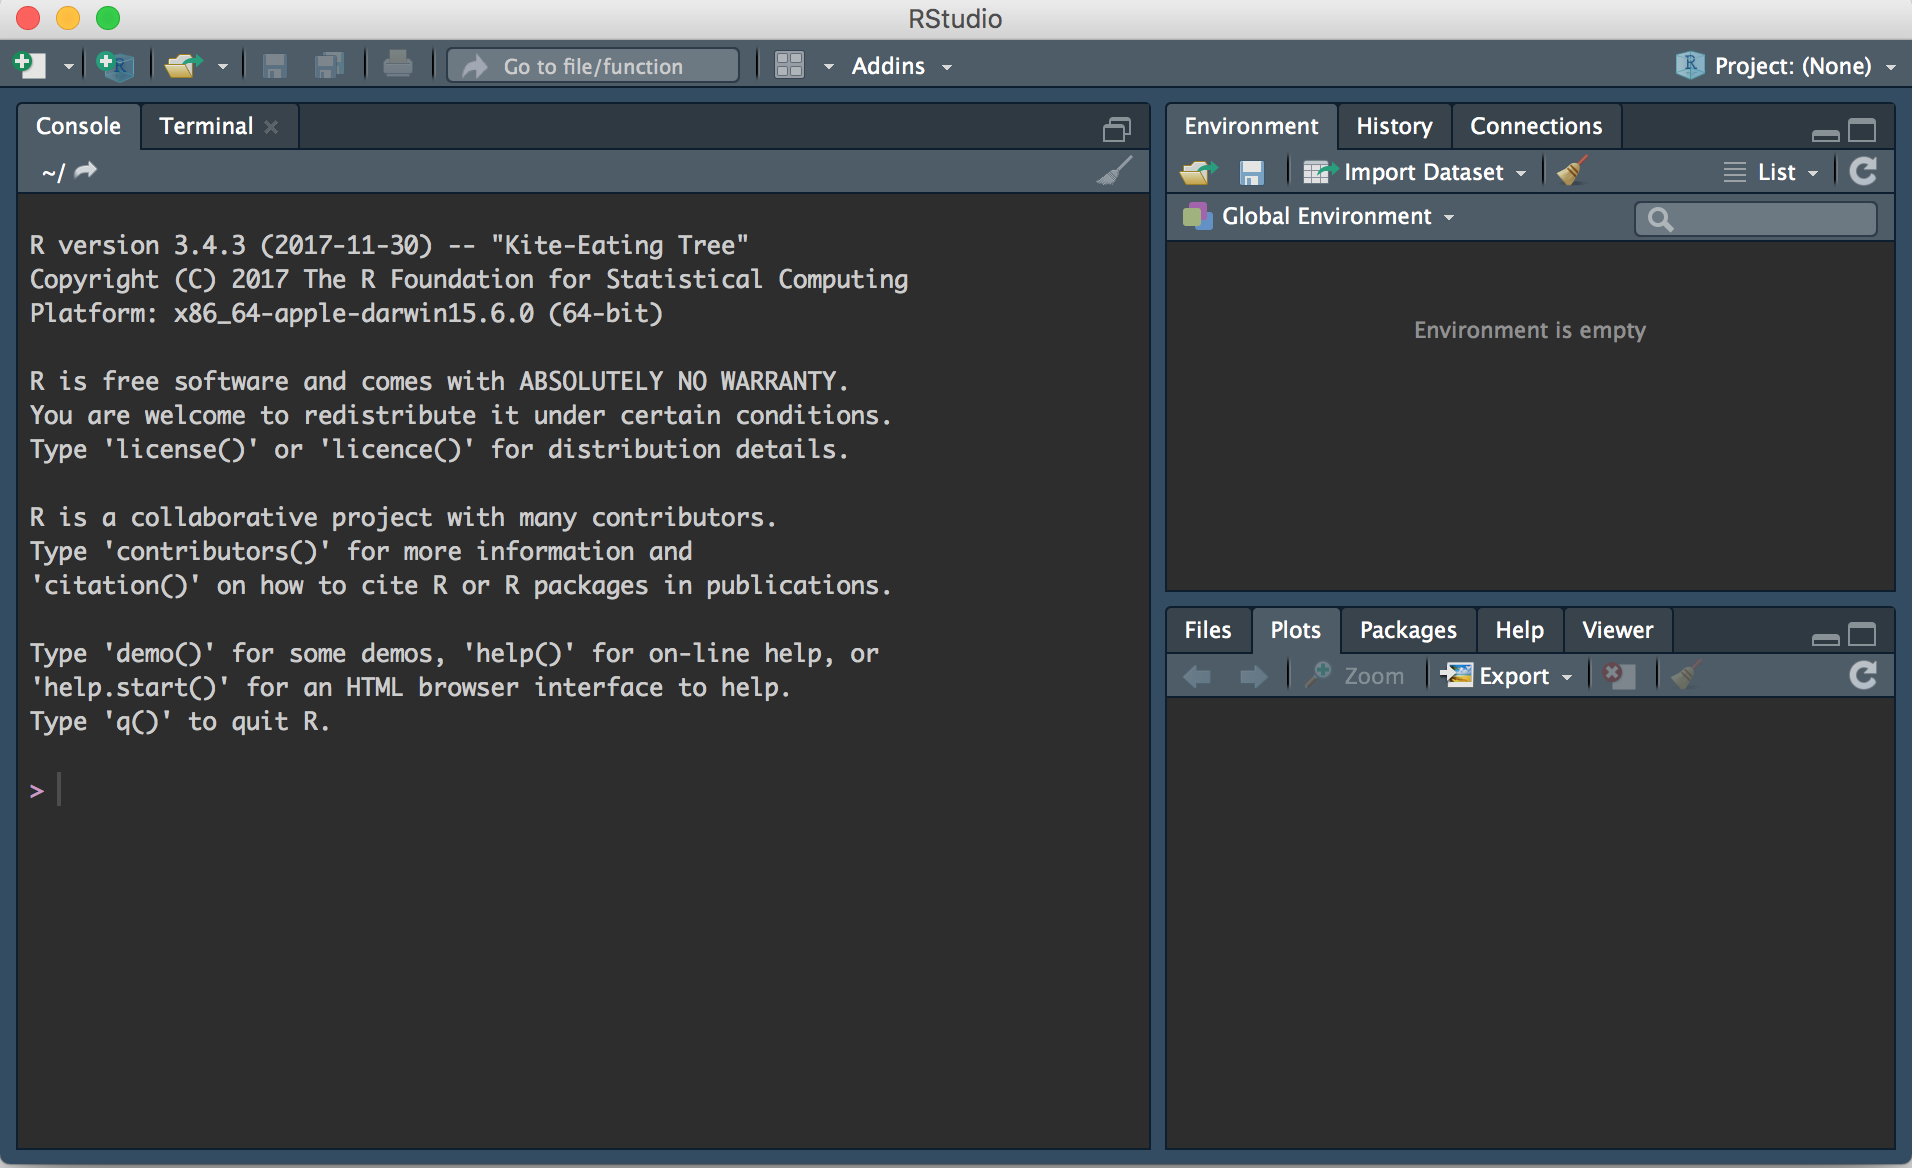
\includegraphics[width=1\linewidth]{fig/rstudio} \caption{Graphical interface in RStudio}\label{fig:interface}
  \end{figure}
  There are three different windows. However, one is missing, and that is
  the window where you will write most of your scripts. You can get this
  window by going to the top menu and select \texttt{File} \(\rightarrow\)
  \texttt{New\ File} \(\rightarrow\) \texttt{R\ Script}. This should give
  you four windows as shown in Figure \ref{fig:interfaceexplain}.
  \begin{figure}
  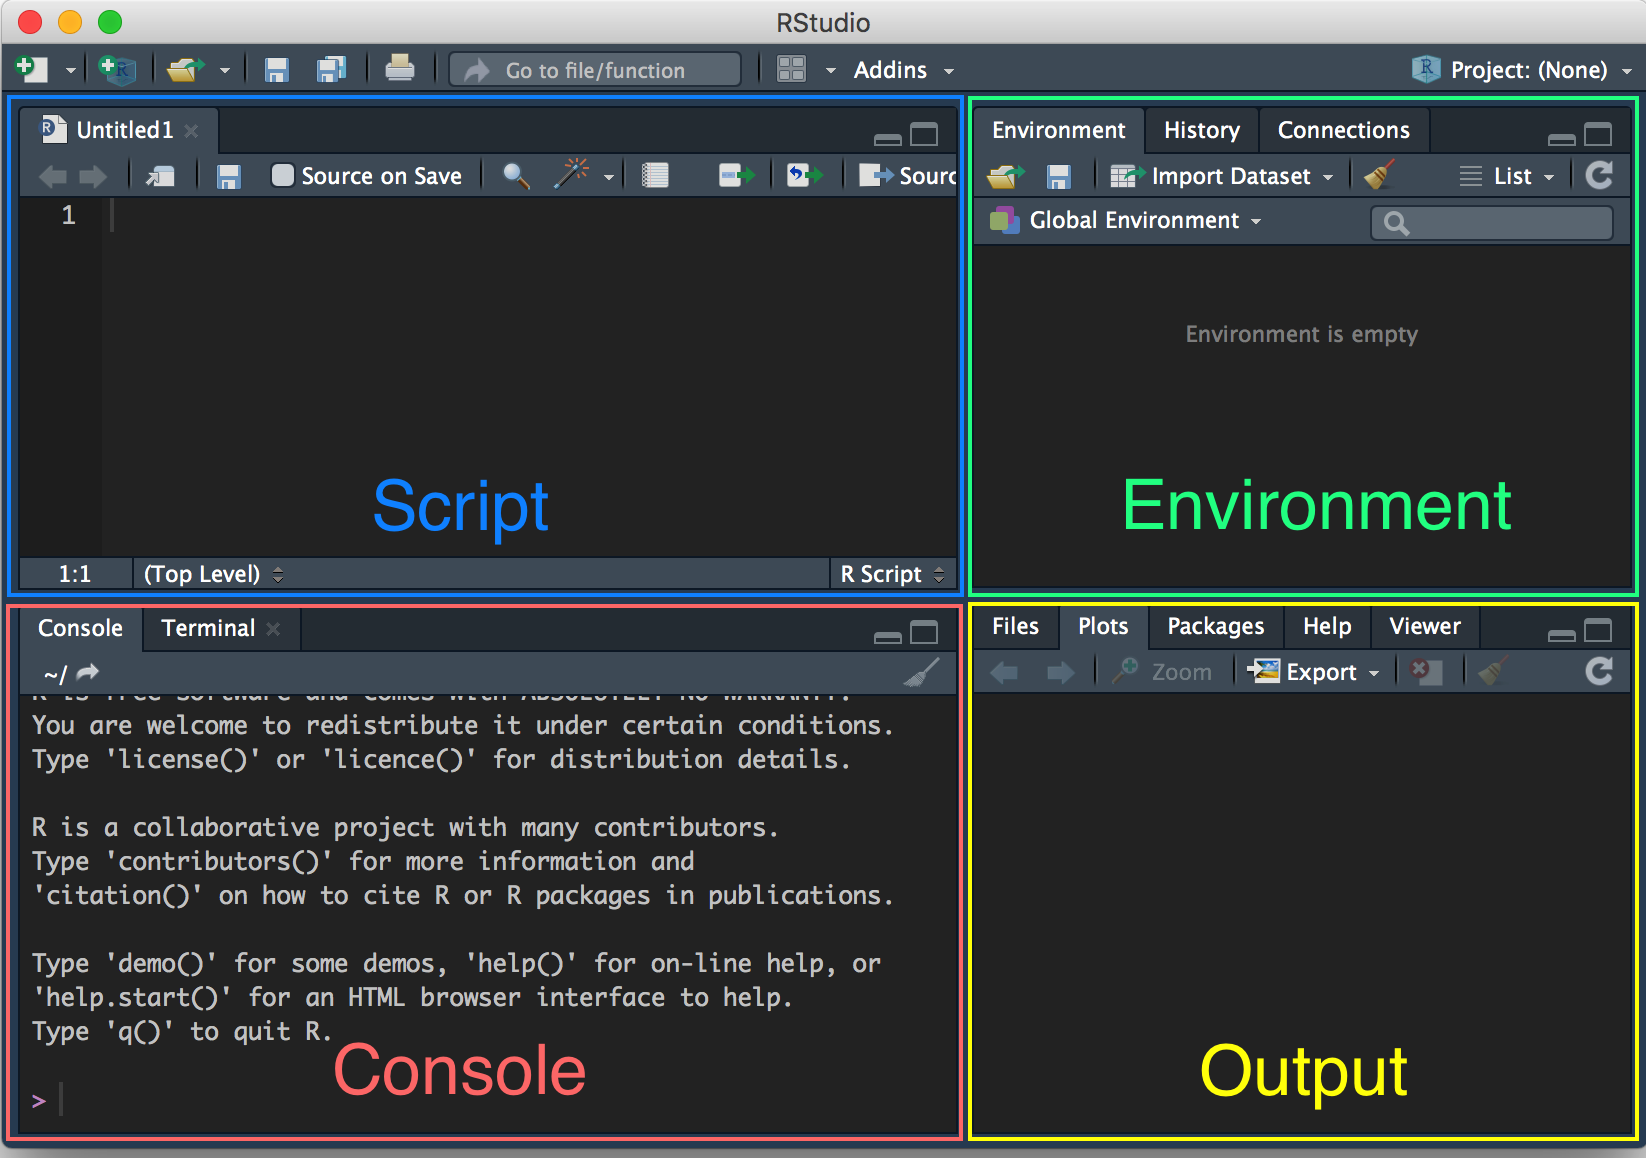
\includegraphics[width=1\linewidth]{fig/rstudio_env} \caption{Graphical interface in RStudio, explained}\label{fig:interfaceexplain}
  \end{figure}
  In the figure, we have emphasized the four windows: script, environment,
  output, and console. The \emph{script} is where you will have your
  \texttt{R} code and make changes. The \emph{environment} is where you
  can see what datasets, variables and other parts you have loaded into R.
  The \emph{output} is where you can see figures you create. The
  \emph{console} is where you can see some output and run commands.
  
  Everything you do in \texttt{R} can be written as commands. This ensures
  that you will always be able to document your work (in your script). In
  the console, you can see a prompt (\texttt{\textgreater{}}). Here, you
  can write what what you want \texttt{R} to do. Try to write \texttt{2+2}
  and hit \texttt{Enter}. This should look like this:
  \begin{Shaded}
  \begin{Highlighting}[]
  \DecValTok{2}\OperatorTok{+}\DecValTok{2}
  \end{Highlighting}
  \end{Shaded}
  \begin{verbatim}
  [1] 4
  \end{verbatim}
  The code you have entered in the console cannot be traced later.
  Accordingly, you will have to save the commands you want to keep in the
  script. Even better, you should write your commands in the script and
  ``run'' them from there. If you write \texttt{2+2} in the script, you
  can mark it and press \texttt{CTRL+R} (Windows) or \texttt{CMD+ENTER}
  (Mac). Then it will run the part of the script that is marked in the
  console. Insert the code below in your script and run it in the console:
  \begin{Shaded}
  \begin{Highlighting}[]
  \DecValTok{50}\OperatorTok{*}\DecValTok{149}
  \DecValTok{3}\OperatorTok{**}\DecValTok{2}        \CommentTok{# 3^2}
  \DecValTok{2}\OperatorTok{**}\DecValTok{3}        \CommentTok{# 2^3}
  \KeywordTok{sqrt}\NormalTok{(}\DecValTok{81}\NormalTok{)    }\CommentTok{# 81^0.5}
  \end{Highlighting}
  \end{Shaded}
  As you can see, we have used \texttt{\#} as well. The \texttt{\#} sign
  tells \texttt{R} that everything after that sign on that line shouldn't
  be read as code but as a comment. In other words, you can write comments
  in your script that will help you remember what you are doing - and help
  others understand the meaning of your script. For now, remember to
  document everything you do in your script.
  
  Notice also that we use a function in the bottom, namely
  \texttt{sqrt()}. A lot of what we will be doing in \texttt{R} is with
  functions. For example, to calculate a mean later we will use the
  \texttt{mean()} function. In the next section we will use functions to
  install and load packages.
  
  \section{\texorpdfstring{Installing \texttt{R}
  packages}{Installing R packages}}\label{installing-r-packages}
  
  We highlighted above that one of the key advantages of using \texttt{R}
  is the package system. In \texttt{R}, a package is a collection of data
  and functions that makes it easier for you do to what you want. The sky
  is the limit and the only thing you need to learn know is how to install
  and load packages.
  
  To install packages, you will have to use a function called
  \texttt{install.packages()}. We will install a package that installs a
  lot of the functions we will be using to manipulate and visualise data.
  More specifically, we will work within the tidyverse (Hadley Wickham,
  2017). You can read more at \href{http://tidyverse.org/}{tidyverse.org}.
  To intall this package type:
  \begin{Shaded}
  \begin{Highlighting}[]
  \KeywordTok{install.packages}\NormalTok{(}\StringTok{"tidyverse"}\NormalTok{)}
  \end{Highlighting}
  \end{Shaded}
  You only need to install the package once. In other words, when you have
  used \texttt{install.packages()} to install a packagae, you will not
  need to install that specific package again. Note that we put
  \texttt{tidyverse} in quotation marks. This is important when you
  install a package. If you forget this, you will get an error.
  
  While you only need to install a package once, you need to load the
  package every time you open \texttt{R}. This is a good thing as you
  don't want to have all your installed \texttt{R} packages working at the
  same time. For this reason, most scripts begin with loading the packages
  that is needed. To load a package, we use the function
  \texttt{library()}:
  \begin{Shaded}
  \begin{Highlighting}[]
  \KeywordTok{library}\NormalTok{(}\StringTok{"tidyverse"}\NormalTok{)}
  \end{Highlighting}
  \end{Shaded}
  To recap, it is always a good idea to begin your script with the
  package(s) you will be working with. If we want to have a script where
  we load the \texttt{tidyverse} package and have some of the commands we
  ran above, the script could look like the script presented in Figure
  \ref{fig:interfacescript}.
  \begin{figure}
  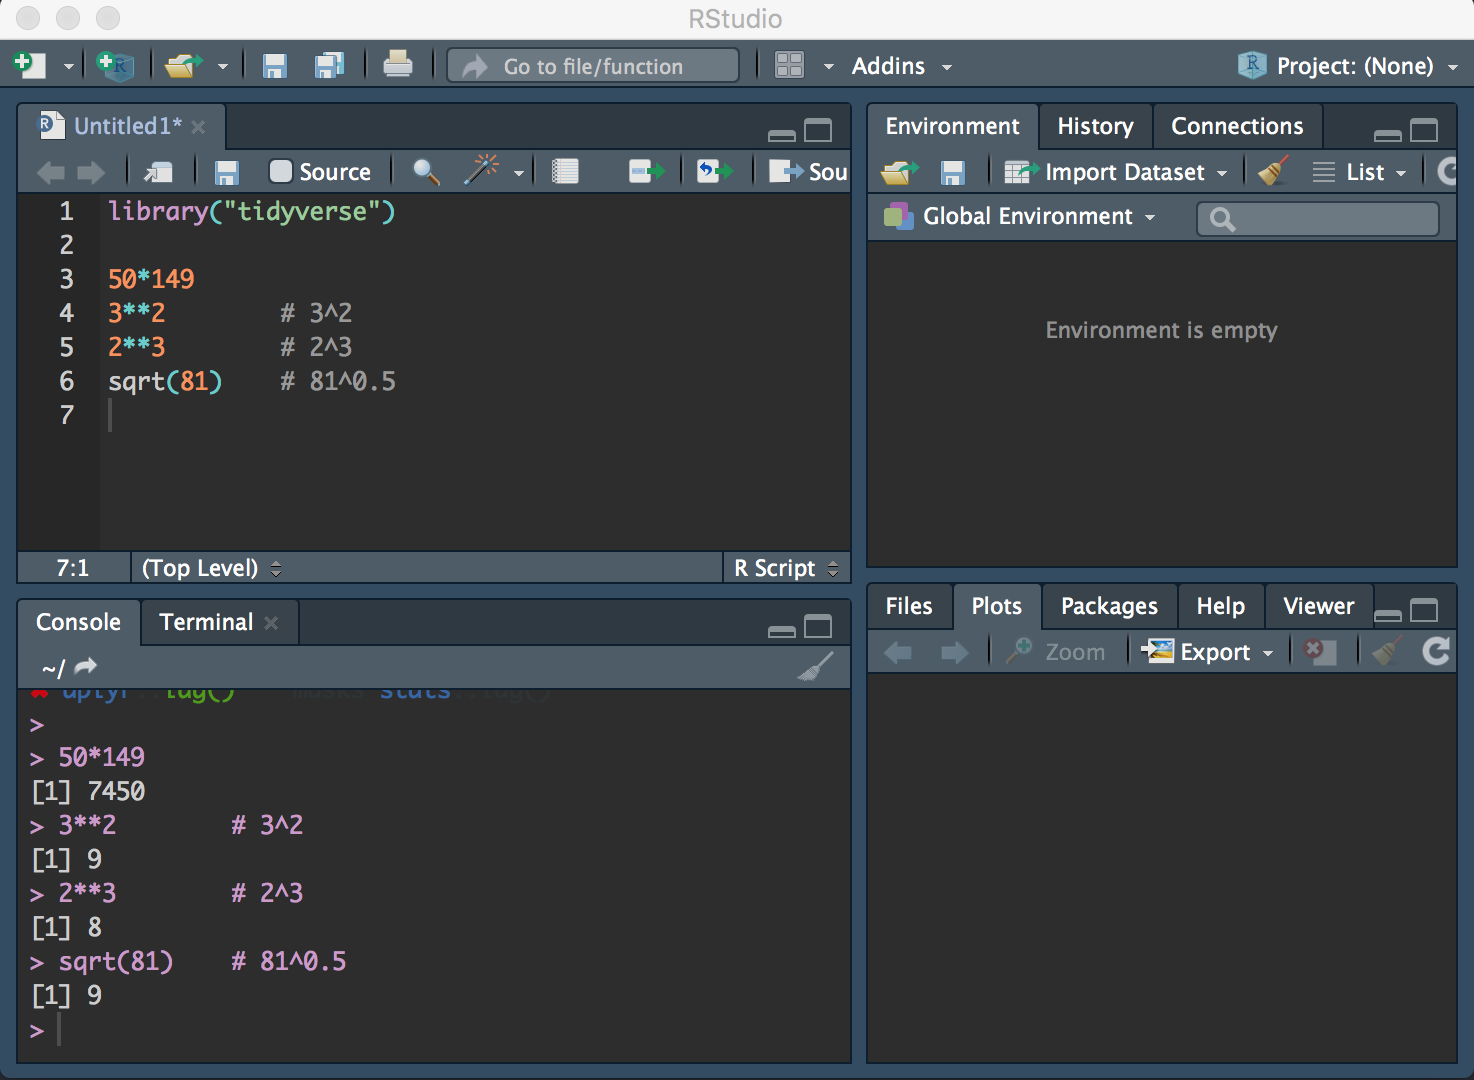
\includegraphics[width=1\linewidth]{fig/rstudio_script} \caption{A script in RStudio}\label{fig:interfacescript}
  \end{figure}
  If you want to save your script you can select \texttt{File}
  \(\rightarrow\) \texttt{Save}, where you can pick a destination for your
  script.
  
  \section{Errors and help}\label{errors-and-help}
  
  As noted above, you will encounter problems and issues when you do stuff
  in \texttt{R}. Sadly, there are many potential reasons to why your
  script might not be working. Your version of \texttt{R} or/and RStudio
  might be too old or too new, you might be using a function that has a
  mistake, you might not have the data in the right format etc.
  
  Consequently, we cannot provide a comprehensive list of errors you might
  get. The best thing to do is to learn how to find help online. Here, the
  best advice is to use Google and, when you search for help, always
  remember to mention R in your search string, and, if you are having
  problems with a specific package, also the name of the package.
  
  \chapter{Basics}\label{basics}
  
  Remember that everything you do in \texttt{R} can be written as
  commands. Repeat what you did in last chapter from your script window:
  write \texttt{2+2} and run the code. This should look like this:
  \begin{Shaded}
  \begin{Highlighting}[]
  \DecValTok{2}\OperatorTok{+}\DecValTok{2}
  \end{Highlighting}
  \end{Shaded}
  \begin{verbatim}
  [1] 4
  \end{verbatim}
  You are now able to conduct simple arithmetics. This shows that
  \texttt{R} can be used as a calculatur and you can now call yourself an
  \texttt{R} user. In other words, knowing how to use \texttt{R} is not a
  binary category where you either can use \texttt{R} or not, but a
  continuum where you will always be able to learn more. That's great
  news!
  
  \section{Numbers as data}\label{numbers-as-data}
  
  Next, we will have to learn about variable assignment and in particular
  how we can work with \emph{objects}. Everything you will use in
  \texttt{R} is saved in objects. This can be everything from a number or
  a word to complex datasets. A key advantage of this compared to other
  statistical programmes is that you can have multiple datasets open at
  the same time. If you, for exampel, want to connect two different
  surveys, you can have them both loaded at the same time. This is not
  possible in SPSS and Stata.
  
  To save something in an objet, we need to use the \emph{assignment
  operator}, \texttt{\textless{}-}, which basically tells \texttt{R} that
  anything on the right side of the operator should be assigned to the
  object on the left side. Let us try to save the number 2 in the object
  \texttt{x}
  \begin{Shaded}
  \begin{Highlighting}[]
  \NormalTok{x <-}\StringTok{ }\DecValTok{2}
  \end{Highlighting}
  \end{Shaded}
  Now \texttt{x} will return the number 2 whenever we use \texttt{x}. Let
  us try to use our object in different simple operations. Write the
  operations in your R-script and run them individually and see what
  happens.
  \begin{Shaded}
  \begin{Highlighting}[]
  \NormalTok{x}
  \NormalTok{x }\OperatorTok{*}\StringTok{ }\DecValTok{2}
  \NormalTok{x }\OperatorTok{*}\StringTok{ }\NormalTok{x }
  \NormalTok{x }\OperatorTok{+}\StringTok{ }\NormalTok{x}
  \end{Highlighting}
  \end{Shaded}
  If it is working, \texttt{R} should return the values \texttt{2},
  \texttt{4}, \texttt{4} and \texttt{4}. If you change the object
  \texttt{x} to have the number 3 instead of 2 and run the script again,
  you should get a new output.\footnote{More specifically, \texttt{3},
    \texttt{6}, \texttt{9} and \texttt{6}.} This is great as you only need
  to change a single number to change the whole procedure. Accordingly,
  when you are working with scripts, try to save as much you can in
  objects, so you only need to change numbers once, if you want to make
  changes. This also reduces the likelihood of you making a mistake.
  
  We can also use our object to create other objects. In the example below
  we will create a new object \texttt{y}. This object returns the sum of
  \texttt{x} and 7.
  \begin{Shaded}
  \begin{Highlighting}[]
  \NormalTok{y <-}\StringTok{ }\NormalTok{x }\OperatorTok{+}\StringTok{ }\DecValTok{7}
  \end{Highlighting}
  \end{Shaded}
  One thing to keep in mind is that we do not get the output in \texttt{y}
  right away. To get the output, we can just write \texttt{y}, or we can,
  when we create the object, include it all in a parenthesis as we do
  below.
  \begin{Shaded}
  \begin{Highlighting}[]
  \NormalTok{(y <-}\StringTok{ }\NormalTok{x }\OperatorTok{+}\StringTok{ }\DecValTok{7}\NormalTok{)}
  \end{Highlighting}
  \end{Shaded}
  \begin{verbatim}
  [1] 9
  \end{verbatim}
  Luckily, we are not limited to save only one number in an object. On the
  contrary, in most objects we will be working with, we will have multiple
  numbers. The code below will return a row of numbers from 1 to 10.
  \begin{Shaded}
  \begin{Highlighting}[]
  \DecValTok{1}\OperatorTok{:}\DecValTok{10}
  \end{Highlighting}
  \end{Shaded}
  \begin{verbatim}
   [1]  1  2  3  4  5  6  7  8  9 10
  \end{verbatim}
  We can save this row of numbers in an object (using
  \texttt{\textless{}-}), but we can also use them directly, e.g.~by
  taking every number in the row and add 2 to all of them.
  \begin{Shaded}
  \begin{Highlighting}[]
  \DecValTok{1}\OperatorTok{:}\DecValTok{10} \OperatorTok{+}\StringTok{ }\DecValTok{2}
  \end{Highlighting}
  \end{Shaded}
  \begin{verbatim}
   [1]  3  4  5  6  7  8  9 10 11 12
  \end{verbatim}
  When you will be working with more numbers, you have to tell \texttt{R},
  that you are working with multiple numbers. To do this, we use the
  function \texttt{c()}. This tells \texttt{R} that we are working with a
  vector.\footnote{In the example with \texttt{1:10}, this is similar to
    writing \texttt{c(1,\ 2,\ 3,\ 4,\ 5,\ 6,\ 7,\ 8,\ 9,\ 10)}. In other
    words, we have a hidden \texttt{c()} when we type \texttt{1:10}.} The
  function \texttt{c()} is short for \emph{concatenate} or
  \emph{combine}.\footnote{\texttt{c()} creates a vector with \emph{all}
    elements in the parenthesis. Since a vector can only have one type of
    data, and not both numbers and text (cf.~next section), \texttt{c()}
    will ensure that all values are reduced to the level all values can
    work with. Consequently, if just one value is a letter and not a
    number, all values in the vector will be considered text.} Remember
  that everything that happens in \texttt{R} happens with functions. A
  vector looks like this:
  \begin{Shaded}
  \begin{Highlighting}[]
  \KeywordTok{c}\NormalTok{(}\DecValTok{2}\NormalTok{, }\DecValTok{2}\NormalTok{, }\DecValTok{2}\NormalTok{)}
  \end{Highlighting}
  \end{Shaded}
  \begin{verbatim}
  [1] 2 2 2
  \end{verbatim}
  This is a \emph{numerical} vector. Again, a vector is a collection of
  values of the same type. We can save any vector in an object without any
  problems. In the code below we save four numbers (14, 6, 23, 2) in the
  object \texttt{x}.
  \begin{Shaded}
  \begin{Highlighting}[]
  \NormalTok{x <-}\StringTok{ }\KeywordTok{c}\NormalTok{(}\DecValTok{14}\NormalTok{, }\DecValTok{6}\NormalTok{, }\DecValTok{23}\NormalTok{, }\DecValTok{2}\NormalTok{)}
  \NormalTok{x}
  \end{Highlighting}
  \end{Shaded}
  \begin{verbatim}
  [1] 14  6 23  2
  \end{verbatim}
  We can then use this vector to calculate new numbers (just as we did
  above with \texttt{1:10}), for example by multiplying all the numbers in
  the vector with 2.
  \begin{Shaded}
  \begin{Highlighting}[]
  \NormalTok{x }\OperatorTok{*}\StringTok{ }\DecValTok{2}
  \end{Highlighting}
  \end{Shaded}
  \begin{verbatim}
  [1] 28 12 46  4
  \end{verbatim}
  If we are only interested in a single value from the vector, we can get
  this value by using brackets, i.e. \texttt{{[}\ {]}}, which you place
  just after the object (so no space between the name of the object and
  the brackets!). By placing the number 3 in the brackets we can get the
  third number in the object.
  \begin{Shaded}
  \begin{Highlighting}[]
  \NormalTok{x[}\DecValTok{3}\NormalTok{]}
  \end{Highlighting}
  \end{Shaded}
  \begin{verbatim}
  [1] 23
  \end{verbatim}
  As you can see, we get the third element, 23. We can use the same
  procedure to get all values with the exception of one value by including
  a negative sign in the brackets. In this example we will get all values
  except for 2. Also, note that since we are not assigned anything to an
  object (with \texttt{\textless{}-}), we are not making any changes to
  \texttt{x}.
  \begin{Shaded}
  \begin{Highlighting}[]
  \NormalTok{x[}\OperatorTok{-}\DecValTok{2}\NormalTok{]}
  \end{Highlighting}
  \end{Shaded}
  \begin{verbatim}
  [1] 14 23  2
  \end{verbatim}
  Now we can try to use a series of functions on our object. The functions
  below will return different types of information such as the number of
  values, the median, the mean, the standard deviation etc.
  \begin{Shaded}
  \begin{Highlighting}[]
  \KeywordTok{length}\NormalTok{(x)     }\CommentTok{# length of vector, number of values}
  \KeywordTok{min}\NormalTok{(x)        }\CommentTok{# minima value}
  \KeywordTok{max}\NormalTok{(x)        }\CommentTok{# maxima value}
  \KeywordTok{median}\NormalTok{(x)     }\CommentTok{# the median}
  \KeywordTok{sum}\NormalTok{(x)        }\CommentTok{# the sum}
  \KeywordTok{mean}\NormalTok{(x)       }\CommentTok{# the mean}
  \KeywordTok{var}\NormalTok{(x)        }\CommentTok{# the variance}
  \KeywordTok{sd}\NormalTok{(x)         }\CommentTok{# the standard deviation}
  \end{Highlighting}
  \end{Shaded}
  The functions should return the values 4, 2, 23, 10, 45, 11.25, 86.25
  and 9.287088.
  
  If we for some reason wants to add an extra number to our vector
  \texttt{x}, we can either create a new vector with all the numbers or
  just overwrite the existing vector with the addition of an extra number:
  \begin{Shaded}
  \begin{Highlighting}[]
  \NormalTok{x <-}\StringTok{ }\KeywordTok{c}\NormalTok{(x, }\DecValTok{5}\NormalTok{)}
  \NormalTok{x}
  \end{Highlighting}
  \end{Shaded}
  \begin{verbatim}
  [1] 14  6 23  2  5
  \end{verbatim}
  We now have five values in our vector instead of four. The value 5 has
  the last place in the vector but if we had added 5 before \texttt{x} in
  the code above, 5 would have been in the beginning of the vector.
  
  Try to use the \texttt{mean()} function on the new object \texttt{x}
  \begin{Shaded}
  \begin{Highlighting}[]
  \KeywordTok{mean}\NormalTok{(x)}
  \end{Highlighting}
  \end{Shaded}
  \begin{verbatim}
  [1] 10
  \end{verbatim}
  Now the mean is 10 (before we added the value 5 to the object the mean
  was 11.25).
  
  \section{\texorpdfstring{Missing values
  (\texttt{NA})}{Missing values (NA)}}\label{missing-values-na}
  
  Up until now we have been lucky that all our ``data'' has been easy to
  work with. However, in the real world - and thereby for most of the data
  we will work with - we will encounter missing values. In Stata you will
  see that missing values gets a dot (`.'). In \texttt{R}, all missing
  values are denoted \texttt{NA}. Let us try to add a missing value to our
  object \texttt{x} and take the mean.
  \begin{Shaded}
  \begin{Highlighting}[]
  \NormalTok{x <-}\StringTok{ }\KeywordTok{c}\NormalTok{(x, }\OtherTok{NA}\NormalTok{)}
  
  \KeywordTok{mean}\NormalTok{(x) }
  \end{Highlighting}
  \end{Shaded}
  \begin{verbatim}
  [1] NA
  \end{verbatim}
  We do not get a mean now but just \texttt{NA}. The reason for this is
  that \texttt{R} is unable to calculate the mean of a vector with a
  missing value included. In order for \texttt{R} to calculate the mean
  now, we need to specifcy that it should remove the missing values before
  calculating the mean. To do this, we add \texttt{na.rm=TRUE} as an
  \emph{option} to the function. Most functions have a series of options
  (more about this later), and the default option for the \texttt{mean()}
  function is not to ignore the missing values.
  \begin{Shaded}
  \begin{Highlighting}[]
  \KeywordTok{mean}\NormalTok{(x, }\DataTypeTok{na.rm=}\OtherTok{TRUE}\NormalTok{)}
  \end{Highlighting}
  \end{Shaded}
  \begin{verbatim}
  [1] 10
  \end{verbatim}
  Now we get the same mean as before we added \texttt{NA} to the object.
  
  \section{Logical operators}\label{logical-operators}
  
  In \texttt{R} a lot of what we will be doing is using logical operators,
  e.g.~testing whether something is equal or similar to something else.
  This is in particular relevant when we have to recode objects and only
  use specific values. If something is true, we get the value
  \texttt{TRUE}, and if something is false, we get \texttt{FALSE}. Try to
  run the code below and see what information you get (and whether it
  makes sense).
  \begin{Shaded}
  \begin{Highlighting}[]
  \NormalTok{x <-}\StringTok{ }\DecValTok{2}
  
  \NormalTok{x }\OperatorTok{==}\StringTok{ }\DecValTok{2}        \CommentTok{# equal to}
  \NormalTok{x }\OperatorTok{==}\StringTok{ }\DecValTok{3}        
  \NormalTok{x }\OperatorTok{!=}\StringTok{ }\DecValTok{2}        \CommentTok{# not equal to}
  \NormalTok{x }\OperatorTok{<}\StringTok{ }\DecValTok{1}         \CommentTok{# less than}
  \NormalTok{x }\OperatorTok{>}\StringTok{ }\DecValTok{1}         \CommentTok{# greater than}
  \NormalTok{x }\OperatorTok{<=}\StringTok{ }\DecValTok{2}        \CommentTok{# less or equal to}
  \NormalTok{x }\OperatorTok{>=}\StringTok{ }\FloatTok{2.01}     \CommentTok{# greater or equal to}
  \end{Highlighting}
  \end{Shaded}
  The script will return \texttt{TRUE}, \texttt{FALSE}, \texttt{FALSE},
  \texttt{FALSE}, \texttt{TRUE}, \texttt{TRUE} and \texttt{FALSE}. If you
  change \texttt{x} to 3, the script will return other values.
  
  \section{Text as data}\label{text-as-data}
  
  In addition to numbers we can also work with text. The difference
  between text and numbers in \texttt{R} is that we use quotation marks to
  indicate that something is text (and not an object).\footnote{Alternatively,
    you can use ' instead of ``. If you want more information on when you
    should use ' instead of'', see
    \url{http://style.tidyverse.org/syntax.html\#quotes}.} As an example,
  we will create an object called \texttt{p} with the political parties
  from the United Kingdom general election in 2017.
  \begin{Shaded}
  \begin{Highlighting}[]
  \NormalTok{p <-}\StringTok{ }\KeywordTok{c}\NormalTok{(}\StringTok{"Conservative Party"}\NormalTok{, }\StringTok{"Labour Party"}\NormalTok{, }\StringTok{"Scottish National Party"}\NormalTok{, }
         \StringTok{"Liberal Democrats"}\NormalTok{, }\StringTok{"Democratic Unionist Party"}\NormalTok{, }\StringTok{"Sinn Féin"}\NormalTok{) }
  
  \NormalTok{p}
  \end{Highlighting}
  \end{Shaded}
  \begin{verbatim}
  [1] "Conservative Party"        "Labour Party"             
  [3] "Scottish National Party"   "Liberal Democrats"        
  [5] "Democratic Unionist Party" "Sinn Féin"                
  \end{verbatim}
  To see what type of data we have in our object, \texttt{p}, we can use
  the function \texttt{class()}. This function returns information on the
  type of data we are having in the object. If we use the function on
  \texttt{p}, we can see that the object consists of characters (i.e.
  \emph{``character''}).
  \begin{Shaded}
  \begin{Highlighting}[]
  \KeywordTok{class}\NormalTok{(p)}
  \end{Highlighting}
  \end{Shaded}
  \begin{verbatim}
  [1] "character"
  \end{verbatim}
  To compare, we can do the same thing with our object \texttt{x}, which
  includes numerical values. Here we see that the function
  \texttt{class()} for \texttt{x} returns \texttt{"numeric"}. The
  different classes a vector can have is: \texttt{character} (text),
  \texttt{numeric} (numbers), \texttt{integer} (whole numbers),
  \texttt{factor} (categories) and \texttt{logical} (logical).
  \begin{Shaded}
  \begin{Highlighting}[]
  \KeywordTok{class}\NormalTok{(x)}
  \end{Highlighting}
  \end{Shaded}
  \begin{verbatim}
  [1] "numeric"
  \end{verbatim}
  To test whether our object is numerical or not, we can use the function
  \texttt{is.numeric()}. If the object is numeric, we will get a
  \texttt{TRUE}. If not, we will get a \texttt{FALSE}. This logical
  structure can be used in a lot of different scenarios as we will see
  later. Similar to \texttt{is.numeric()}, we have a function called
  \texttt{is.character()} that will show us whether the object is a
  charater or not.
  \begin{Shaded}
  \begin{Highlighting}[]
  \KeywordTok{is.numeric}\NormalTok{(x)}
  \KeywordTok{is.character}\NormalTok{(x)}
  \end{Highlighting}
  \end{Shaded}
  Try to use \texttt{is.numeric()} and \texttt{is.character()} on the
  object \texttt{p}.
  
  In the same way we could get specific values from the object when it was
  numeric, we can get specific values when it is a character object as
  well.
  \begin{Shaded}
  \begin{Highlighting}[]
  \NormalTok{p[}\DecValTok{3}\NormalTok{]}
  \end{Highlighting}
  \end{Shaded}
  \begin{verbatim}
  [1] "Scottish National Party"
  \end{verbatim}
  \begin{Shaded}
  \begin{Highlighting}[]
  \NormalTok{p[}\OperatorTok{-}\DecValTok{3}\NormalTok{]}
  \end{Highlighting}
  \end{Shaded}
  \begin{verbatim}
  [1] "Conservative Party"        "Labour Party"             
  [3] "Liberal Democrats"         "Democratic Unionist Party"
  [5] "Sinn Féin"                
  \end{verbatim}
  While \texttt{p} is a short name for an object and easy to write, it is
  not telling for what we actually have in the object. Accordingly, let us
  create a new object called \texttt{party} with the same information as
  in \texttt{p}. When you name objects remember that they are case
  sensitive so \texttt{party} will be a different object than
  \texttt{Party}.\footnote{If you want more information on how to name
    objects, see
    \url{http://style.tidyverse.org/syntax.html\#object-names}.}
  \begin{Shaded}
  \begin{Highlighting}[]
  \NormalTok{party <-}\StringTok{ }\NormalTok{p}
  
  \NormalTok{party}
  \end{Highlighting}
  \end{Shaded}
  \begin{verbatim}
  [1] "Conservative Party"        "Labour Party"             
  [3] "Scottish National Party"   "Liberal Democrats"        
  [5] "Democratic Unionist Party" "Sinn Féin"                
  \end{verbatim}
  \section{Data frames}\label{data-frames}
  
  In most cases, we will not be working with one variable
  (e.g.~information on party names), but multiple variables. To do this in
  an easy way, we can create \emph{data frames} which is similar to a
  dataset in SPSS and Stata. The good thing about \texttt{R}, however, is
  that we can have multiple data frames open at the same time. The cost of
  this is that we have to specifcy, when we do something in \texttt{R},
  exactly what data frame we are using.
  
  Here we will create a data frame with more information about the parties
  from the United Kingdom general election, 2017.\footnote{The information
    is taken from
    \url{https://en.wikipedia.org/wiki/United_Kingdom_general_election,_2017}}
  
  As a first step we can create new objects with more information:
  \texttt{leader} (ifnormation on the party leader), \texttt{votes} (the
  vote share in percent), \texttt{seats} (the number of seats) and
  \texttt{seats\_change} (change in seats from the previous election). Do
  note that the order is important as we are going to link these objects
  together in a minute, where the first value in each object is for the
  Conservative Party, the second for the Labour Party and so on.
  \begin{Shaded}
  \begin{Highlighting}[]
  \NormalTok{leader <-}\StringTok{ }\KeywordTok{c}\NormalTok{(}\StringTok{"Theresa May"}\NormalTok{, }\StringTok{"Jeremy Corbyn"}\NormalTok{, }\StringTok{"Nicola Sturgeon"}\NormalTok{, }
              \StringTok{"Tim Farron"}\NormalTok{, }\StringTok{"Arlene Foster"}\NormalTok{, }\StringTok{"Gerry Adams"}\NormalTok{)}
  \NormalTok{votes <-}\StringTok{ }\KeywordTok{c}\NormalTok{(}\FloatTok{42.4}\NormalTok{, }\FloatTok{40.0}\NormalTok{, }\FloatTok{3.0}\NormalTok{, }\FloatTok{7.4}\NormalTok{, }\FloatTok{0.9}\NormalTok{, }\FloatTok{0.7}\NormalTok{)}
  \NormalTok{seats <-}\StringTok{ }\KeywordTok{c}\NormalTok{(}\DecValTok{317}\NormalTok{, }\DecValTok{262}\NormalTok{, }\DecValTok{35}\NormalTok{, }\DecValTok{12}\NormalTok{, }\DecValTok{10}\NormalTok{, }\DecValTok{7}\NormalTok{)}
  \NormalTok{seats_change <-}\StringTok{ }\KeywordTok{c}\NormalTok{(}\OperatorTok{-}\DecValTok{13}\NormalTok{, }\DecValTok{30}\NormalTok{, }\OperatorTok{-}\DecValTok{21}\NormalTok{, }\DecValTok{4}\NormalTok{, }\DecValTok{2}\NormalTok{, }\DecValTok{3}\NormalTok{)}
  \end{Highlighting}
  \end{Shaded}
  The next thing we have to do is to connect the objects into a single
  object, i.e.~our data frame. A data frame is a collection of different
  vectors of the same length. In other words, for the objects we have
  above, as they have the same number of information, they can be
  connected in a data frame. \texttt{R} will return an error message if
  the vectors do not have the same length.
  
  We can have different types of variables in a data frame, i.e.~both
  numbers and text variables. To create our data frame, we will use the
  function \texttt{data.frame()} and save the data frame in the object
  \texttt{uk2017}.
  \begin{Shaded}
  \begin{Highlighting}[]
  \NormalTok{uk2017 <-}\StringTok{ }\KeywordTok{data.frame}\NormalTok{(party, leader, votes, seats, seats_change)}
  
  \NormalTok{uk2017 }\CommentTok{# show the content of the data frame}
  \end{Highlighting}
  \end{Shaded}
  \begin{verbatim}
                        party          leader votes seats seats_change
  1        Conservative Party     Theresa May  42.4   317          -13
  2              Labour Party   Jeremy Corbyn  40.0   262           30
  3   Scottish National Party Nicola Sturgeon   3.0    35          -21
  4         Liberal Democrats      Tim Farron   7.4    12            4
  5 Democratic Unionist Party   Arlene Foster   0.9    10            2
  6                 Sinn Féin     Gerry Adams   0.7     7            3
  \end{verbatim}
  To see what type of object we are working with, we can use the function
  \texttt{class()} to show that \texttt{uk2017} is a data frame.
  \begin{Shaded}
  \begin{Highlighting}[]
  \KeywordTok{class}\NormalTok{(uk2017)}
  \end{Highlighting}
  \end{Shaded}
  \begin{verbatim}
  [1] "data.frame"
  \end{verbatim}
  If we would like to know what class the individual variables in our data
  frame are, we can use the function \texttt{sapply()}. This function
  allows us to apply a function to a list or a vector. Below we apply
  \texttt{class()} on the individual variables in \texttt{uk2017}.
  \begin{Shaded}
  \begin{Highlighting}[]
  \KeywordTok{sapply}\NormalTok{(uk2017, class)}
  \end{Highlighting}
  \end{Shaded}
  \begin{verbatim}
         party       leader        votes        seats seats_change 
      "factor"     "factor"    "numeric"    "numeric"    "numeric" 
  \end{verbatim}
  Here we can see that we have data as a \texttt{factor} as well as
  numerical variables. We can get similar information about our data by
  using the function \texttt{str()}. This function returns information on
  the structure in the data frame.
  \begin{Shaded}
  \begin{Highlighting}[]
  \KeywordTok{str}\NormalTok{(uk2017)}
  \end{Highlighting}
  \end{Shaded}
  \begin{verbatim}
  'data.frame':   6 obs. of  5 variables:
   $ party       : Factor w/ 6 levels "Conservative Party",..: 1 3 5 4 2 6
   $ leader      : Factor w/ 6 levels "Arlene Foster",..: 5 3 4 6 1 2
   $ votes       : num  42.4 40 3 7.4 0.9 0.7
   $ seats       : num  317 262 35 12 10 7
   $ seats_change: num  -13 30 -21 4 2 3
  \end{verbatim}
  Here we can see that it is a data frame with 6 observations of 5
  variables. If the rows (i.e.~observations) have names, we can get these
  by using \texttt{rownames()}. We can get the names of the columns,
  i.e.~the variables in our data frame, by using \texttt{colnames()}.
  \begin{Shaded}
  \begin{Highlighting}[]
  \KeywordTok{colnames}\NormalTok{(uk2017)}
  \end{Highlighting}
  \end{Shaded}
  \begin{verbatim}
  [1] "party"        "leader"       "votes"        "seats"       
  [5] "seats_change"
  \end{verbatim}
  If we want to see the number of columns and rows in our data frame, we
  can use \texttt{ncol()} and \texttt{nrow()}.
  \begin{Shaded}
  \begin{Highlighting}[]
  \KeywordTok{ncol}\NormalTok{(uk2017)}
  \end{Highlighting}
  \end{Shaded}
  \begin{verbatim}
  [1] 5
  \end{verbatim}
  \begin{Shaded}
  \begin{Highlighting}[]
  \KeywordTok{nrow}\NormalTok{(uk2017)}
  \end{Highlighting}
  \end{Shaded}
  \begin{verbatim}
  [1] 6
  \end{verbatim}
  If we are working with bigger data frames, e.g.~a survey with thousands
  of respondents, it might not be useful to just show the full data frame.
  One way to see just a few of the observations is by using
  \texttt{head()}. If not specified further, this function will show the
  first six observations in the data frame. In the example below, we will
  tell \texttt{R} to show the first three observations
  \begin{Shaded}
  \begin{Highlighting}[]
  \KeywordTok{head}\NormalTok{(uk2017, }\DecValTok{3}\NormalTok{)  }\CommentTok{# show the first three rows}
  \end{Highlighting}
  \end{Shaded}
  \begin{verbatim}
                      party          leader votes seats seats_change
  1      Conservative Party     Theresa May  42.4   317          -13
  2            Labour Party   Jeremy Corbyn  40.0   262           30
  3 Scottish National Party Nicola Sturgeon   3.0    35          -21
  \end{verbatim}
  In the same way, we can use \texttt{tail()} show the last observations
  in a data frame. Here we see the last four observations in our data
  frame.
  \begin{Shaded}
  \begin{Highlighting}[]
  \KeywordTok{tail}\NormalTok{(uk2017, }\DecValTok{4}\NormalTok{)  }\CommentTok{# show the last four rows}
  \end{Highlighting}
  \end{Shaded}
  \begin{verbatim}
                        party          leader votes seats seats_change
  3   Scottish National Party Nicola Sturgeon   3.0    35          -21
  4         Liberal Democrats      Tim Farron   7.4    12            4
  5 Democratic Unionist Party   Arlene Foster   0.9    10            2
  6                 Sinn Féin     Gerry Adams   0.7     7            3
  \end{verbatim}
  If you want to see your data frame in a new window, you can use the
  function \texttt{View()} (do note the capital letter V - not v).
  \begin{Shaded}
  \begin{Highlighting}[]
  \KeywordTok{View}\NormalTok{(uk2017)}
  \end{Highlighting}
  \end{Shaded}
  \begin{figure}
  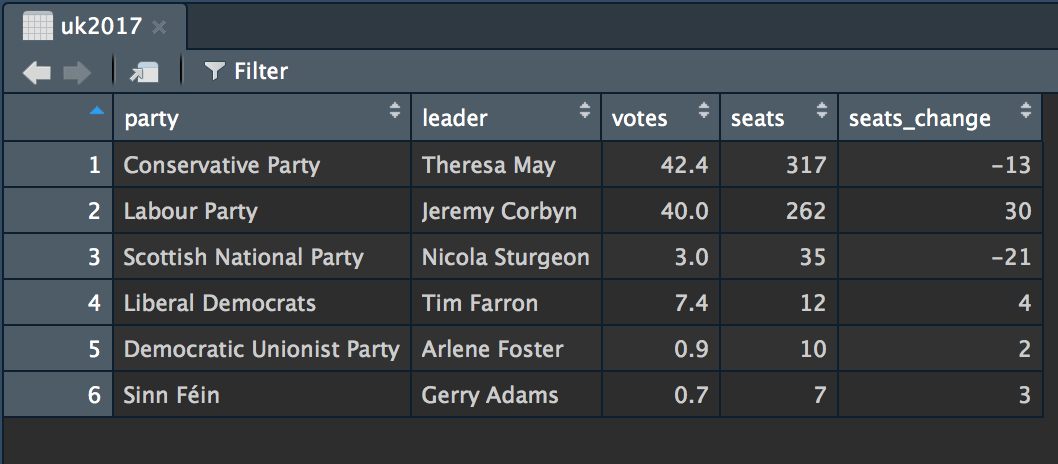
\includegraphics[scale=0.65]{fig/View} \caption{Data frame with View(), RStudio}\label{fig:View}
  \end{figure}
  When you are working with variables in a data frame, you can use
  \texttt{\$} as a \emph{component selector} to select a variable in a
  data frame. This is the base R way, i.e.~brackets and dollar signs. In
  the next chapter we will work with other functions that makes it easier
  to work with data frames.
  
  If we, for example, want to have all the vote shares in our data frame
  \texttt{uk2017}, we can write \texttt{uk2017\$votes}.
  \begin{Shaded}
  \begin{Highlighting}[]
  \NormalTok{uk2017}\OperatorTok{$}\NormalTok{votes}
  \end{Highlighting}
  \end{Shaded}
  \begin{verbatim}
  [1] 42.4 40.0  3.0  7.4  0.9  0.7
  \end{verbatim}
  Contrary to working with a vector in a single dimension, we have two
  dimensions in a data frame (rows horisontally and columns vertically).
  Just as for a single vector, we need to work with the brackets,
  \texttt{{[}\ {]}}, in addition to our object, but we need to specify the
  rows and columns we are interested in. If we want to work with the first
  row, we need to specify \texttt{{[}1,\ {]}} after the object. The comma
  is seperating the information on the rows and columns we want to work
  with. When we are not specifying anything after the comma, that means we
  want to have the information for \emph{all} columns.
  \begin{Shaded}
  \begin{Highlighting}[]
  \NormalTok{uk2017[}\DecValTok{1}\NormalTok{,] }\CommentTok{# first row}
  \end{Highlighting}
  \end{Shaded}
  \begin{verbatim}
                 party      leader votes seats seats_change
  1 Conservative Party Theresa May  42.4   317          -13
  \end{verbatim}
  Had we also added a number after the comma, we would get the information
  for that specific column. in the example below we want to have the
  information on the first row in the first column (i.e.~the name of the
  party on the first row).
  \begin{Shaded}
  \begin{Highlighting}[]
  \NormalTok{uk2017[}\DecValTok{1}\NormalTok{, }\DecValTok{1}\NormalTok{] }\CommentTok{# first row, first column}
  \end{Highlighting}
  \end{Shaded}
  \begin{verbatim}
  [1] Conservative Party
  6 Levels: Conservative Party Democratic Unionist Party ... Sinn Féin
  \end{verbatim}
  If we want to have the names of all parties, i.e.~the information in the
  first column, we can specify that we want all rows but only for the
  first column.
  \begin{Shaded}
  \begin{Highlighting}[]
  \NormalTok{uk2017[, }\DecValTok{1}\NormalTok{] }\CommentTok{# first column}
  \end{Highlighting}
  \end{Shaded}
  \begin{verbatim}
  [1] Conservative Party        Labour Party             
  [3] Scottish National Party   Liberal Democrats        
  [5] Democratic Unionist Party Sinn Féin                
  6 Levels: Conservative Party Democratic Unionist Party ... Sinn Féin
  \end{verbatim}
  Interestingly, the functions we have talked about so far can all be
  applied to data frames. The \texttt{summary()} function is very useful
  if you want to get an overview of all your variables in your data frame.
  For the numerical variables in the data frame, the function will return
  information such as the mean and the median.
  \begin{Shaded}
  \begin{Highlighting}[]
  \KeywordTok{summary}\NormalTok{(uk2017)}
  \end{Highlighting}
  \end{Shaded}
  \begin{verbatim}
                         party               leader      votes       
   Conservative Party       :1   Arlene Foster  :1   Min.   : 0.700  
   Democratic Unionist Party:1   Gerry Adams    :1   1st Qu.: 1.425  
   Labour Party             :1   Jeremy Corbyn  :1   Median : 5.200  
   Liberal Democrats        :1   Nicola Sturgeon:1   Mean   :15.733  
   Scottish National Party  :1   Theresa May    :1   3rd Qu.:31.850  
   Sinn Féin                :1   Tim Farron     :1   Max.   :42.400  
       seats        seats_change     
   Min.   :  7.0   Min.   :-21.0000  
   1st Qu.: 10.5   1st Qu.: -9.2500  
   Median : 23.5   Median :  2.5000  
   Mean   :107.2   Mean   :  0.8333  
   3rd Qu.:205.2   3rd Qu.:  3.7500  
   Max.   :317.0   Max.   : 30.0000  
  \end{verbatim}
  We can also use the functions on our variables as we did above, e.g.~to
  get the maximum number of votes a party got with the function
  \texttt{max()}.
  \begin{Shaded}
  \begin{Highlighting}[]
  \KeywordTok{max}\NormalTok{(uk2017}\OperatorTok{$}\NormalTok{votes)}
  \end{Highlighting}
  \end{Shaded}
  \begin{verbatim}
  [1] 42.4
  \end{verbatim}
  If we want to have the value on a specific variable in our data frame,
  we can use both \texttt{\$} and \texttt{{[}\ {]}}. Below we get the
  second value in the variable \texttt{party}.
  \begin{Shaded}
  \begin{Highlighting}[]
  \NormalTok{uk2017}\OperatorTok{$}\NormalTok{party[}\DecValTok{2}\NormalTok{]}
  \end{Highlighting}
  \end{Shaded}
  \begin{verbatim}
  [1] Labour Party
  6 Levels: Conservative Party Democratic Unionist Party ... Sinn Féin
  \end{verbatim}
  To combine a lot of what we have used above, we can get informatin on
  the name of the party that got the most votes. In order to do this, we
  specify that we would like to have the name of the party for the party
  where the number of votes equals the maximum number of votes. In other
  words, when \texttt{uk2017\$votes} is equal to
  \texttt{max(uk2017\$votes)}, we want to get the information on
  \texttt{uk2017\$party}. We use \texttt{==} to test whether something is
  equal to.
  \begin{Shaded}
  \begin{Highlighting}[]
  \NormalTok{uk2017}\OperatorTok{$}\NormalTok{party[uk2017}\OperatorTok{$}\NormalTok{votes }\OperatorTok{==}\StringTok{ }\KeywordTok{max}\NormalTok{(uk2017}\OperatorTok{$}\NormalTok{votes)]}
  \end{Highlighting}
  \end{Shaded}
  \begin{verbatim}
  [1] Conservative Party
  6 Levels: Conservative Party Democratic Unionist Party ... Sinn Féin
  \end{verbatim}
  As we can see, the Conservative Party got the most votes in the 2017
  election. We can use the same procedure if we want to get information on
  the party that got the minimum number of votes. To do this we use
  \texttt{min()}. Here we can see that this is Sinn Féin in our data
  frame.
  \begin{Shaded}
  \begin{Highlighting}[]
  \NormalTok{uk2017}\OperatorTok{$}\NormalTok{party[uk2017}\OperatorTok{$}\NormalTok{votes }\OperatorTok{==}\StringTok{ }\KeywordTok{min}\NormalTok{(uk2017}\OperatorTok{$}\NormalTok{votes)]}
  \end{Highlighting}
  \end{Shaded}
  \begin{verbatim}
  [1] Sinn Féin
  6 Levels: Conservative Party Democratic Unionist Party ... Sinn Féin
  \end{verbatim}
  The sky is the limit when it comes t owhat we can do with data frames,
  including various types of statistical analyses. To give one example, we
  can use the \texttt{lm()} function to conduct an OLS regression with
  \texttt{votes} as the independent variable and \texttt{seats} as the
  dependent variable. First, we save the model in the object
  \texttt{uk2017\_lm} and then use \texttt{summary()} to get the results.
  \begin{Shaded}
  \begin{Highlighting}[]
  \NormalTok{uk2017_lm <-}\StringTok{ }\KeywordTok{lm}\NormalTok{(seats }\OperatorTok{~}\StringTok{ }\NormalTok{votes, }\DataTypeTok{data =}\NormalTok{ uk2017)}
  
  \KeywordTok{summary}\NormalTok{(uk2017_lm)}
  \end{Highlighting}
  \end{Shaded}
  \begin{verbatim}
  
  Call:
  lm(formula = seats ~ votes, data = uk2017)
  
  Residuals:
        1       2       3       4       5       6 
   20.890 -17.105  18.054 -36.122   7.933   6.350 
  
  Coefficients:
              Estimate Std. Error t value Pr(>|t|)    
  (Intercept)   -4.310     13.405  -0.321 0.763932    
  votes          7.085      0.558  12.698 0.000222 ***
  ---
  Signif. codes:  0 '***' 0.001 '**' 0.01 '*' 0.05 '.' 0.1 ' ' 1
  
  Residual standard error: 24.81 on 4 degrees of freedom
  Multiple R-squared:  0.9758,    Adjusted R-squared:  0.9697 
  F-statistic: 161.2 on 1 and 4 DF,  p-value: 0.0002216
  \end{verbatim}
  \section{Import and export data
  frames}\label{import-and-export-data-frames}
  
  Most of the data frames we will be working with in \texttt{R} are not
  data frames we will build from scratch but on the contrary data frames
  we will import from other files such as files made for Stata, SPSS or
  Excel. The most useful filetype to use when you work with data in files
  is \texttt{.csv}, which stands for \emph{comma-separated values}. This
  is an open file format and be opened in any software. To export and
  import data frames to \texttt{.csv} files, we can use
  \texttt{write.csv()} and \texttt{read.csv()}.
  
  First of all we need to know where \texttt{R} is working from, i.e.~what
  our \emph{working directory} is. To get this you can type
  \texttt{getwd()} and see where your data will be saved.
  \begin{Shaded}
  \begin{Highlighting}[]
  \KeywordTok{getwd}\NormalTok{()}
  \end{Highlighting}
  \end{Shaded}
  If you would like to change this, you can use the function
  \texttt{setwd()}. This function allows you to change the working
  directory to whatever folder on your computer you would like to use.
  \begin{Shaded}
  \begin{Highlighting}[]
  \KeywordTok{setwd}\NormalTok{(}\StringTok{"/Dropbox/qpolr/book"}\NormalTok{)}
  \end{Highlighting}
  \end{Shaded}
  An easy way to control the working directory is to open an R-script
  directly from the folder so it also opens RStudio that way. This will
  automatically set the working directory to the folder with the R-script.
  
  Once we know where we will save our data, we can use
  \texttt{write.csv()} to save the data. In the code below we first
  specify that we want to save the data frame \texttt{uk2017} and next the
  filename of the file (\texttt{uk2017.csv}).
  \begin{Shaded}
  \begin{Highlighting}[]
  \KeywordTok{write.csv}\NormalTok{(uk2017, }\StringTok{"uk2017.csv"}\NormalTok{)}
  \end{Highlighting}
  \end{Shaded}
  Do note that we need to put the file in quotation marks. Next, we can
  import the file into \texttt{R} the next time we open \texttt{R} with
  the function \texttt{read.csv()} and save the data frame in the object
  \texttt{uk2017}.
  \begin{Shaded}
  \begin{Highlighting}[]
  \NormalTok{uk2017 <-}\StringTok{ }\KeywordTok{read.csv}\NormalTok{(}\StringTok{"uk2017.csv"}\NormalTok{)}
  \end{Highlighting}
  \end{Shaded}
  As with most stuff in \texttt{R}, there are multiple ways of doing
  things. To import and export data, we have packages like
  \texttt{foreign} (R Core Team, 2015), \texttt{rio} (C. Chan, Chan, \&
  Leeper, 2016) og \texttt{readr} (H. Wickham \& Francois, 2015). If you
  install and load the package \texttt{rio}, you can use the functions
  \texttt{import()} and \texttt{export()}.
  \begin{Shaded}
  \begin{Highlighting}[]
  \CommentTok{# export data with the rio package}
  \KeywordTok{export}\NormalTok{(uk2017, }\StringTok{"uk2017.csv"}\NormalTok{)}
  
  \CommentTok{# import data with the rio package}
  \NormalTok{uk2017 <-}\StringTok{ }\KeywordTok{import}\NormalTok{(}\StringTok{"uk2017.csv"}\NormalTok{)}
  \end{Highlighting}
  \end{Shaded}
  \section{Environment}\label{environment}
  
  We have worked with a series of different objects. T osee what objects
  we have in our memory, we can look in the \emph{Environment} window, but
  we can also use the function \texttt{ls()}(\emph{ls} is short for
  \emph{list objects}).
  \begin{Shaded}
  \begin{Highlighting}[]
  \KeywordTok{ls}\NormalTok{()}
  \end{Highlighting}
  \end{Shaded}
  \begin{verbatim}
   [1] "leader"       "p"            "party"        "seats"       
   [5] "seats_change" "uk2017"       "uk2017_lm"    "votes"       
   [9] "x"            "y"           
  \end{verbatim}
  If we would like to remove an object from the memory, we can use the
  function \texttt{rm()} (\emph{rm} is short for \emph{remove}). Below we
  use \texttt{rm()} to remove the object \texttt{x} and then \texttt{ls()}
  to check whether \texttt{x} is gone.
  \begin{Shaded}
  \begin{Highlighting}[]
  \KeywordTok{rm}\NormalTok{(x)}
  
  \KeywordTok{ls}\NormalTok{()}
  \end{Highlighting}
  \end{Shaded}
  \begin{verbatim}
  [1] "leader"       "p"            "party"        "seats"       
  [5] "seats_change" "uk2017"       "uk2017_lm"    "votes"       
  [9] "y"           
  \end{verbatim}
  If you would like to remove \emph{everything} in the memory, you can use
  \texttt{ls()} in combination with \texttt{rm()}.
  \begin{Shaded}
  \begin{Highlighting}[]
  \KeywordTok{rm}\NormalTok{(}\DataTypeTok{list =} \KeywordTok{ls}\NormalTok{())}
  
  \KeywordTok{ls}\NormalTok{()}
  \end{Highlighting}
  \end{Shaded}
  \chapter{Data management}\label{data}
  
  There are multiple ways to manage data in \texttt{R} and in particular
  ways to create and change variables in a data frame. In this chapter, we
  show different ways of working with data frames with a focus on how to
  change variables. Noteworthy, there are multiple packages we can use to
  manipulate data farmes, but the best is without a doubt \texttt{dplyr}
  (Hadley Wickham \& Francois, 2016).
  
  The package provides some basic functions making it easy to work with
  data frames. These functions include \texttt{select()},
  \texttt{filter()}, \texttt{arrange()}, \texttt{rename()},
  \texttt{mutate()} og \texttt{summarize()}.\footnote{For another good
    introduction to \texttt{dplyr}, see:
    \href{https://bookdown.org/rdpeng/rprogdatascience/managing-data-frames-with-the-dplyr-package.html}{Managing
    Data Frames with the dplyr package}.} \texttt{select()} allows you to
  pick variables by their names. \texttt{filter()} allows you to pick
  observations by their values. \texttt{arrange()} allows you to reorder
  the rows. \texttt{rename()} allows you to rename columns.
  \texttt{mutate()} allows you to create new variables based on the values
  of old variables. \texttt{summarize()} allows you to collapse many
  values to a single summary.
  
  All these functions rely on data frames. In other words, you can not use
  these functions on other types of data in \texttt{R}. Furthermore, they
  all return a new data frame.
  
  The \texttt{dplyr} package is a part of the \texttt{tidyverse}. First,
  load the \texttt{tidyverse}.
  \begin{Shaded}
  \begin{Highlighting}[]
  \KeywordTok{library}\NormalTok{(}\StringTok{"tidyverse"}\NormalTok{)}
  \end{Highlighting}
  \end{Shaded}
  We will use the dataset we created in the previous chapter. If you do
  not have it, you can download it here:
  \url{http://qpolr.com/data/uk2017.csv}
  \begin{Shaded}
  \begin{Highlighting}[]
  \NormalTok{uk2017 <-}\StringTok{ }\KeywordTok{import}\NormalTok{(}\StringTok{"uk2017.csv"}\NormalTok{)}
  \end{Highlighting}
  \end{Shaded}
  To see the information in the dataset, use \texttt{head()}.
  \begin{Shaded}
  \begin{Highlighting}[]
  \KeywordTok{head}\NormalTok{(uk2017)}
  \end{Highlighting}
  \end{Shaded}
  \begin{verbatim}
                        party          leader votes seats seats_change
  1        Conservative Party     Theresa May  42.4   317          -13
  2              Labour Party   Jeremy Corbyn  40.0   262           30
  3   Scottish National Party Nicola Sturgeon   3.0    35          -21
  4         Liberal Democrats      Tim Farron   7.4    12            4
  5 Democratic Unionist Party   Arlene Foster   0.9    10            2
  6                 Sinn Féin     Gerry Adams   0.7     7            3
  \end{verbatim}
  \section{\texorpdfstring{Selecting variables:
  \texttt{select()}}{Selecting variables: select()}}\label{selecting-variables-select}
  
  When we work with large datasets, we often want to select the few
  variables that are of key interest to our project. For this, the
  \texttt{select()} function is perfect. If we only want to have
  information on the party name and the votes in the \texttt{uk2017} data
  frame, we can write:
  \begin{Shaded}
  \begin{Highlighting}[]
  \KeywordTok{select}\NormalTok{(uk2017, party, votes)}
  \end{Highlighting}
  \end{Shaded}
  \begin{verbatim}
                        party votes
  1        Conservative Party  42.4
  2              Labour Party  40.0
  3   Scottish National Party   3.0
  4         Liberal Democrats   7.4
  5 Democratic Unionist Party   0.9
  6                 Sinn Féin   0.7
  \end{verbatim}
  There are multiple different functions that can help us finding specific
  variables in the data frame. We can use \texttt{contains()}, if we want
  to include variables that contain a specific word in the variable name.
  In the example below we look for variables that contain \texttt{seat}.
  \begin{Shaded}
  \begin{Highlighting}[]
  \KeywordTok{select}\NormalTok{(uk2017, }\KeywordTok{contains}\NormalTok{(}\StringTok{"seat"}\NormalTok{))}
  \end{Highlighting}
  \end{Shaded}
  \begin{verbatim}
    seats seats_change
  1   317          -13
  2   262           30
  3    35          -21
  4    12            4
  5    10            2
  6     7            3
  \end{verbatim}
  Other noteworthy functions that can be of help similar to
  \texttt{contains()} are functions such as \texttt{starts\_with()},
  \texttt{ends\_with()}, \texttt{matches()}, \texttt{num\_range()},
  \texttt{one\_of()} and \texttt{everything()}. The last function,
  \texttt{everything()} is helpful if we want to move a variable to the
  beginning of our data frame.
  \begin{Shaded}
  \begin{Highlighting}[]
  \KeywordTok{select}\NormalTok{(uk2017, votes, }\KeywordTok{everything}\NormalTok{())}
  \end{Highlighting}
  \end{Shaded}
  \begin{verbatim}
    votes                     party          leader seats seats_change
  1  42.4        Conservative Party     Theresa May   317          -13
  2  40.0              Labour Party   Jeremy Corbyn   262           30
  3   3.0   Scottish National Party Nicola Sturgeon    35          -21
  4   7.4         Liberal Democrats      Tim Farron    12            4
  5   0.9 Democratic Unionist Party   Arlene Foster    10            2
  6   0.7                 Sinn Féin     Gerry Adams     7            3
  \end{verbatim}
  We can use the negative sign if we want to remove a variable from the
  data frame.
  \begin{Shaded}
  \begin{Highlighting}[]
  \KeywordTok{select}\NormalTok{(uk2017, }\OperatorTok{-}\NormalTok{leader)}
  \end{Highlighting}
  \end{Shaded}
  \begin{verbatim}
                        party votes seats seats_change
  1        Conservative Party  42.4   317          -13
  2              Labour Party  40.0   262           30
  3   Scottish National Party   3.0    35          -21
  4         Liberal Democrats   7.4    12            4
  5 Democratic Unionist Party   0.9    10            2
  6                 Sinn Féin   0.7     7            3
  \end{verbatim}
  \section{\texorpdfstring{Selecting observations:
  \texttt{filter()}}{Selecting observations: filter()}}\label{selecting-observations-filter}
  
  To select only some of the observations in our data frame, but for all
  variables, we can use the function \texttt{filter()}. In the example
  below we select the observations in our data frame with a positive value
  on \texttt{seats\_change} (i.e.~greater than 0).
  \begin{Shaded}
  \begin{Highlighting}[]
  \KeywordTok{filter}\NormalTok{(uk2017, seats_change }\OperatorTok{>}\StringTok{ }\DecValTok{0}\NormalTok{)}
  \end{Highlighting}
  \end{Shaded}
  \begin{verbatim}
                        party        leader votes seats seats_change
  1              Labour Party Jeremy Corbyn  40.0   262           30
  2         Liberal Democrats    Tim Farron   7.4    12            4
  3 Democratic Unionist Party Arlene Foster   0.9    10            2
  4                 Sinn Féin   Gerry Adams   0.7     7            3
  \end{verbatim}
  Importantly, we are \emph{not} making any changes to the data frame
  \texttt{uk2017}. This will only hapen if we replace our existing data
  frame or create a new data frame. In the example below we create a new
  data frame, \texttt{uk2017\_seatlosers}, with the observations losing
  seats from 2015 to 2017.
  \begin{Shaded}
  \begin{Highlighting}[]
  \NormalTok{uk2017_seatlosers <-}\StringTok{ }\KeywordTok{filter}\NormalTok{(uk2017, seats_change }\OperatorTok{<}\StringTok{ }\DecValTok{0}\NormalTok{)}
  \NormalTok{uk2017_seatlosers}
  \end{Highlighting}
  \end{Shaded}
  \begin{verbatim}
                      party          leader votes seats seats_change
  1      Conservative Party     Theresa May  42.4   317          -13
  2 Scottish National Party Nicola Sturgeon   3.0    35          -21
  \end{verbatim}
  Last, if we want to drop observations that contain missing values on
  specific variables, we can use the function \texttt{drop\_na()}.
  
  \section{\texorpdfstring{Sorting observations:
  \texttt{arrange()}}{Sorting observations: arrange()}}\label{sorting-observations-arrange}
  
  We can use the function \texttt{arrange()} if we want to change the
  order of observations. In the example below we sort our data frame
  according to how many votes the party got, with the party getting the
  least votes in the top of our data frame.
  \begin{Shaded}
  \begin{Highlighting}[]
  \KeywordTok{arrange}\NormalTok{(uk2017, votes)}
  \end{Highlighting}
  \end{Shaded}
  \begin{verbatim}
                        party          leader votes seats seats_change
  1                 Sinn Féin     Gerry Adams   0.7     7            3
  2 Democratic Unionist Party   Arlene Foster   0.9    10            2
  3   Scottish National Party Nicola Sturgeon   3.0    35          -21
  4         Liberal Democrats      Tim Farron   7.4    12            4
  5              Labour Party   Jeremy Corbyn  40.0   262           30
  6        Conservative Party     Theresa May  42.4   317          -13
  \end{verbatim}
  If we prefer to have the parties with the maximum number of votes in the
  top, we can use the negative sign (\texttt{-}).
  \begin{Shaded}
  \begin{Highlighting}[]
  \KeywordTok{arrange}\NormalTok{(uk2017, }\OperatorTok{-}\NormalTok{votes)}
  \end{Highlighting}
  \end{Shaded}
  \begin{verbatim}
                        party          leader votes seats seats_change
  1        Conservative Party     Theresa May  42.4   317          -13
  2              Labour Party   Jeremy Corbyn  40.0   262           30
  3         Liberal Democrats      Tim Farron   7.4    12            4
  4   Scottish National Party Nicola Sturgeon   3.0    35          -21
  5 Democratic Unionist Party   Arlene Foster   0.9    10            2
  6                 Sinn Féin     Gerry Adams   0.7     7            3
  \end{verbatim}
  \section{\texorpdfstring{Rename variables:
  \texttt{rename()}}{Rename variables: rename()}}\label{rename-variables-rename}
  
  In the case we have a variable we would prefer having another name, we
  can use the function \texttt{rename()}. In the example below we change
  the name of \texttt{party} to \texttt{party\_name}.
  \begin{Shaded}
  \begin{Highlighting}[]
  \KeywordTok{rename}\NormalTok{(uk2017, }\DataTypeTok{party_name =}\NormalTok{ party)}
  \end{Highlighting}
  \end{Shaded}
  \begin{verbatim}
                   party_name          leader votes seats seats_change
  1        Conservative Party     Theresa May  42.4   317          -13
  2              Labour Party   Jeremy Corbyn  40.0   262           30
  3   Scottish National Party Nicola Sturgeon   3.0    35          -21
  4         Liberal Democrats      Tim Farron   7.4    12            4
  5 Democratic Unionist Party   Arlene Foster   0.9    10            2
  6                 Sinn Féin     Gerry Adams   0.7     7            3
  \end{verbatim}
  \section{\texorpdfstring{Create variables:
  \texttt{mutate()}}{Create variables: mutate()}}\label{create-variables-mutate}
  
  The best way to create a new variable from existing variables in our
  data frame is to use the function \texttt{mutate()}. In the example
  below we create a new variable, \texttt{votes\_m} with information on
  how many percentage points a party is from the average number of votes a
  party got.
  \begin{Shaded}
  \begin{Highlighting}[]
  \KeywordTok{mutate}\NormalTok{(uk2017, }\DataTypeTok{votes_m =}\NormalTok{ votes }\OperatorTok{-}\StringTok{ }\KeywordTok{mean}\NormalTok{(votes))}
  \end{Highlighting}
  \end{Shaded}
  \begin{verbatim}
                        party          leader votes seats seats_change
  1        Conservative Party     Theresa May  42.4   317          -13
  2              Labour Party   Jeremy Corbyn  40.0   262           30
  3   Scottish National Party Nicola Sturgeon   3.0    35          -21
  4         Liberal Democrats      Tim Farron   7.4    12            4
  5 Democratic Unionist Party   Arlene Foster   0.9    10            2
  6                 Sinn Féin     Gerry Adams   0.7     7            3
       votes_m
  1  26.666667
  2  24.266667
  3 -12.733333
  4  -8.333333
  5 -14.833333
  6 -15.033333
  \end{verbatim}
  In another example we use the \texttt{sum()} function as well to find
  the proportion of seats a party got in a variable, \texttt{seats\_prop}.
  \begin{Shaded}
  \begin{Highlighting}[]
  \KeywordTok{mutate}\NormalTok{(uk2017, }\DataTypeTok{seats_prop =}\NormalTok{ seats }\OperatorTok{/}\StringTok{ }\KeywordTok{sum}\NormalTok{(seats))}
  \end{Highlighting}
  \end{Shaded}
  \begin{verbatim}
                        party          leader votes seats seats_change
  1        Conservative Party     Theresa May  42.4   317          -13
  2              Labour Party   Jeremy Corbyn  40.0   262           30
  3   Scottish National Party Nicola Sturgeon   3.0    35          -21
  4         Liberal Democrats      Tim Farron   7.4    12            4
  5 Democratic Unionist Party   Arlene Foster   0.9    10            2
  6                 Sinn Féin     Gerry Adams   0.7     7            3
    seats_prop
  1 0.49300156
  2 0.40746501
  3 0.05443235
  4 0.01866252
  5 0.01555210
  6 0.01088647
  \end{verbatim}
  \section{\texorpdfstring{The pipe operator:
  \texttt{\%\textgreater{}\%}}{The pipe operator: \%\textgreater{}\%}}\label{the-pipe-operator}
  
  So far we have looked at a series of different functions. In most cases
  we want to combine these functions, e.g.~when we both have to select
  specific variables and observations. Luckikly, there is nothing against
  using one function nested within another, as the example below shows.
  \begin{Shaded}
  \begin{Highlighting}[]
  \KeywordTok{filter}\NormalTok{(}\KeywordTok{select}\NormalTok{(uk2017, party, votes), seats_change }\OperatorTok{>}\StringTok{ }\DecValTok{0}\NormalTok{)}
  \end{Highlighting}
  \end{Shaded}
  \begin{verbatim}
                        party votes
  1              Labour Party  40.0
  2         Liberal Democrats   7.4
  3 Democratic Unionist Party   0.9
  4                 Sinn Féin   0.7
  \end{verbatim}
  The problem is that it can be complicated to read, especially when as
  the number of functions we use increase. Furthermore, the likelihood of
  making a stupid mistake, e.g.~by including an extra \texttt{(} or
  \texttt{)} increases substantially. Luckily, we can use the pipe
  operator, \texttt{\%\textgreater{}\%}, to make our code more readable.
  
  The operator relies on a step-wise logic so we first specify the data
  frame and then a line for each function we want to run on the data
  frame.
  
  In the example below we do the same as above but in a way that is easier
  to follow.
  \begin{Shaded}
  \begin{Highlighting}[]
  \NormalTok{uk2017 }\OperatorTok\StringTok{ }
  \StringTok{  }\KeywordTok{select}\NormalTok{(party, votes) }\OperatorTok
  \StringTok{  }\KeywordTok{filter}\NormalTok{(seats_change }\OperatorTok{>}\StringTok{ }\DecValTok{0}\NormalTok{)}
  \end{Highlighting}
  \end{Shaded}
  \begin{verbatim}
                        party votes
  1              Labour Party  40.0
  2         Liberal Democrats   7.4
  3 Democratic Unionist Party   0.9
  4                 Sinn Féin   0.7
  \end{verbatim}
  On the first line, we show that we are using the data frame
  \texttt{uk2017}. We end this line with \texttt{\%\textgreater{}\%},
  telling \texttt{R} that we are not done yet but will have to put this
  into the function on the line below. The next line uses the input from
  the previous line and selects \texttt{party} and \texttt{votes} from the
  data frame. This line also ends with the pipe,
  \texttt{\%\textgreater{}\%}. The third line shows the observations in
  our data frame where \texttt{seats\_change} is greater than 0. Note that
  we did not select \texttt{seats\_change} as a variable with
  \texttt{select()}, so this is not crucial in order to use it (as long as
  it is in the \texttt{uk2017} data frame). Last, we do \emph{not} end
  with a pipe as we are now done.
  
  \section{\texorpdfstring{Running functions on variables:
  \texttt{apply()}}{Running functions on variables: apply()}}\label{running-functions-on-variables-apply}
  
  If we would like to run a function on some of our rows or columns we can
  use the function \texttt{apply()}. For example, we can get the average
  number of votes and seats for parties with a positive value on
  \texttt{seats\_change} (i.e.~parties with an increase in seats from 2015
  to 2017.
  
  The addition here is the function \texttt{apply()} on the data frame
  used above. The first thing we specify here is \texttt{MARGIN},
  i.e.~whether we want to run a function on our rows (1) or columns (2).
  The next thing we specify is the function together with any relevant
  options.
  \begin{Shaded}
  \begin{Highlighting}[]
  \NormalTok{uk2017 }\OperatorTok
  \StringTok{  }\KeywordTok{filter}\NormalTok{(seats_change }\OperatorTok{>}\StringTok{ }\DecValTok{0}\NormalTok{) }\OperatorTok
  \StringTok{  }\KeywordTok{select}\NormalTok{(votes, seats) }\OperatorTok
  \StringTok{  }\KeywordTok{apply}\NormalTok{(}\DataTypeTok{MARGIN =} \DecValTok{2}\NormalTok{, }\DataTypeTok{FUN =}\NormalTok{ mean, }\DataTypeTok{na.rm =} \OtherTok{TRUE}\NormalTok{)}
  \end{Highlighting}
  \end{Shaded}
  \begin{verbatim}
  votes seats 
  12.25 72.75 
  \end{verbatim}
  In the case you want to apply a function to both rows and columns, you
  will have to specify \texttt{c(1,\ 2)}. It is not important to mention
  \texttt{MARGIN} eller \texttt{FUN} if you have the order right. In other
  words, we can simplify our example to the code below.
  \begin{Shaded}
  \begin{Highlighting}[]
  \NormalTok{uk2017 }\OperatorTok
  \StringTok{  }\KeywordTok{filter}\NormalTok{(seats_change }\OperatorTok{>}\StringTok{ }\DecValTok{0}\NormalTok{) }\OperatorTok
  \StringTok{  }\KeywordTok{select}\NormalTok{(votes, seats) }\OperatorTok
  \StringTok{  }\KeywordTok{apply}\NormalTok{(}\DecValTok{2}\NormalTok{, mean)}
  \end{Highlighting}
  \end{Shaded}
  \begin{verbatim}
  votes seats 
  12.25 72.75 
  \end{verbatim}
  \section{\texorpdfstring{Aggregating variables: \texttt{summarize()} and
  \texttt{group\_by()}}{Aggregating variables: summarize() and group\_by()}}\label{aggregating-variables-summarize-and-group_by}
  
  If we want to create new variables with aggregated information, similar
  to the information we got in the previous section, we can use the
  function \texttt{summarize()}. In the example below we get a data frame
  with information on the number of observatins, given by \texttt{n()},
  the minimum number of votes a party got (\texttt{votes\_min}), the
  maximum number of votes a party got (\texttt{votes\_max}) and the
  average number of votes a party got (\texttt{votes\_mean}) (all in
  percentages).
  \begin{Shaded}
  \begin{Highlighting}[]
  \NormalTok{uk2017 }\OperatorTok
  \StringTok{  }\KeywordTok{summarize}\NormalTok{(}\DataTypeTok{party =} \KeywordTok{n}\NormalTok{(), }
              \DataTypeTok{votes_min =} \KeywordTok{min}\NormalTok{(votes), }
              \DataTypeTok{votes_max =} \KeywordTok{max}\NormalTok{(votes), }
              \DataTypeTok{votes_mean =} \KeywordTok{mean}\NormalTok{(votes))}
  \end{Highlighting}
  \end{Shaded}
  \begin{verbatim}
    party votes_min votes_max votes_mean
  1     6       0.7      42.4   15.73333
  \end{verbatim}
  If we want this information for different groups, we can supply with
  \texttt{group\_by()}. In the example below we will like to have the
  information both for parties with an increase in seats from 2015 to 2017
  and not.
  \begin{Shaded}
  \begin{Highlighting}[]
  \NormalTok{uk2017 }\OperatorTok
  \StringTok{  }\KeywordTok{group_by}\NormalTok{(seats_change }\OperatorTok{>}\StringTok{ }\DecValTok{0}\NormalTok{) }\OperatorTok
  \StringTok{  }\KeywordTok{summarize}\NormalTok{(}\DataTypeTok{party =} \KeywordTok{n}\NormalTok{(), }
              \DataTypeTok{votes_min =} \KeywordTok{min}\NormalTok{(votes), }
              \DataTypeTok{votes_max =} \KeywordTok{max}\NormalTok{(votes), }
              \DataTypeTok{votes_mean =} \KeywordTok{mean}\NormalTok{(votes))}
  \end{Highlighting}
  \end{Shaded}
  \begin{verbatim}
  # A tibble: 2 x 5
    `seats_change > 0` party votes_min votes_max votes_mean
    <lgl>              <int>     <dbl>     <dbl>      <dbl>
  1 F                      2     3.00       42.4       22.7
  2 T                      4     0.700      40.0       12.2
  \end{verbatim}
  In the example, you can see the aggregated information. \texttt{T} is
  short for \texttt{TRUE} and is the aggregated information for the
  observations where \texttt{seats\_change} is greater than 0.
  
  \section{\texorpdfstring{Recoding variables:
  \texttt{recode()}}{Recoding variables: recode()}}\label{recoding-variables-recode}
  
  In a lot of cases we want to recode the information in a single
  variable. To do this, we can use \texttt{recode()}. Importantly, this
  function works for individual variables and not for a data frame. Let us
  use the \texttt{leader} variable in \texttt{uk2017} as an example.
  \begin{Shaded}
  \begin{Highlighting}[]
  \NormalTok{uk2017}\OperatorTok{$}\NormalTok{leader }
  \end{Highlighting}
  \end{Shaded}
  \begin{verbatim}
  [1] Theresa May     Jeremy Corbyn   Nicola Sturgeon Tim Farron     
  [5] Arlene Foster   Gerry Adams    
  6 Levels: Arlene Foster Gerry Adams Jeremy Corbyn ... Tim Farron
  \end{verbatim}
  In the case that we want to replace Tim Farron in the variable with a
  new guy, we can do that with the code below.
  \begin{Shaded}
  \begin{Highlighting}[]
  \KeywordTok{recode}\NormalTok{(uk2017}\OperatorTok{$}\NormalTok{leader, }\StringTok{"Tim Farron"}\NormalTok{ =}\StringTok{ "New guy"}\NormalTok{)}
  \end{Highlighting}
  \end{Shaded}
  \begin{verbatim}
  [1] Theresa May     Jeremy Corbyn   Nicola Sturgeon New guy        
  [5] Arlene Foster   Gerry Adams    
  6 Levels: Arlene Foster Gerry Adams Jeremy Corbyn ... New guy
  \end{verbatim}
  Noteworthy, we do not create any changes to the \texttt{leader}
  variable. If we want to save the changes, we can save the new variable
  to our data frame.
  \begin{Shaded}
  \begin{Highlighting}[]
  \NormalTok{uk2017}\OperatorTok{$}\NormalTok{leader_new <-}\StringTok{ }\KeywordTok{recode}\NormalTok{(uk2017}\OperatorTok{$}\NormalTok{leader, }\StringTok{"Tim Farron"}\NormalTok{ =}\StringTok{ "New guy"}\NormalTok{)}
  
  \NormalTok{uk2017}\OperatorTok{$}\NormalTok{leader_new}
  \end{Highlighting}
  \end{Shaded}
  \begin{verbatim}
  [1] Theresa May     Jeremy Corbyn   Nicola Sturgeon New guy        
  [5] Arlene Foster   Gerry Adams    
  6 Levels: Arlene Foster Gerry Adams Jeremy Corbyn ... New guy
  \end{verbatim}
  Last, \texttt{dplyr} in the \texttt{tidyverse} is not the only package
  with a \texttt{recode()} function. The package \texttt{car} (Fox \&
  Weisberg, 2011) has a similar function worth exploring.
  
  \backmatter
  
  \chapter{References}\label{references}
  
  \noindent
  
  \setlength{\parindent}{-0.20in} \setlength{\leftskip}{0.20in}
  \setlength{\parskip}{8pt}
  
  \hypertarget{refs}{}
  \hypertarget{ref-chanetal2016}{}
  Chan, C., Chan, G. C. H., \& Leeper, T. J. (2016). \emph{Rio: A
  swiss-army knife for data file i/o}.
  
  \hypertarget{ref-foxweisberg2011}{}
  Fox, J., \& Weisberg, S. (2011). \emph{An R companion to applied
  regression} (Second). Thousand Oaks CA: Sage. Retrieved from
  \url{http://socserv.socsci.mcmaster.ca/jfox/Books/Companion}
  
  \hypertarget{ref-rcoreteam2015foreign}{}
  R Core Team. (2015). \emph{Foreign: Read data stored by minitab, s, sas,
  spss, stata, systat, weka, dBase, ...} Retrieved from
  \url{http://CRAN.R-project.org/package=foreign}
  
  \hypertarget{ref-wickham2017}{}
  Wickham, H. (2017). \emph{Tidyverse: Easily install and load the
  'tidyverse'}. Retrieved from
  \url{https://CRAN.R-project.org/package=tidyverse}
  
  \hypertarget{ref-wickhamfrancois2015}{}
  Wickham, H., \& Francois, R. (2015). \emph{Readr: Read tabular data}.
  Retrieved from \url{http://CRAN.R-project.org/package=readr}
  
  \hypertarget{ref-wickhamfrancois2016}{}
  Wickham, H., \& Francois, R. (2016). \emph{Dplyr: A grammar of data
  manipulation}. Retrieved from
  \url{http://CRAN.R-project.org/package=dplyr}


  % Index?

\end{document}
